\chapter{Quá trình thực hiện}
\label{Chapter4}

% ============================================================
\section{Giới thiệu khái quát}
% ============================================================
Trong quá trình thực hiện đề tài, nhóm đã sử dụng một số công cụ hỗ trợ nhằm đảm bảo quá trình phát triển diễn ra có tổ chức, hiệu quả và dễ dàng cộng tác. Các công cụ được lựa chọn dựa trên nhiều tiêu chí như: sự quen thuộc và kinh nghiệm sử dụng trước đó của các thành viên, tính năng phong phú đáp ứng nhu cầu của nhóm, cũng như mức độ phổ biến trong cộng đồng phát triển phần mềm hiện nay.
 
Cụ thể, các công cụ được nhóm sử dụng bao gồm:
 
\begin{itemize}
    \item \textbf{Jira}: Được sử dụng để quản lý công việc (task management), theo dõi tiến độ các sprint và phân công nhiệm vụ cho từng thành viên.
 
    \item \textbf{GitHub}: Được sử dụng để quản lý mã nguồn (source control). Nhóm tổ chức thành 3 repository riêng biệt: một cho back-end, một cho front-end web và một cho front-end mobile. GitHub cũng được sử dụng trong quy trình tạo pull request và review code.
 
    \item \textbf{draw.io}: Được sử dụng để thiết kế các sơ đồ kiến trúc hệ thống, sơ đồ luồng dữ liệu và các biểu đồ kỹ thuật khác.
 
    \item \textbf{Google Meet}: Được sử dụng làm nền tảng họp trực tuyến hàng tuần giữa các thành viên trong nhóm cũng như giữa nhóm và giáo viên hướng dẫn.
 
    \item \textbf{Google Drive}: Được sử dụng để lưu trữ và chia sẻ tài liệu chung của nhóm như biên bản họp, tài liệu đặc tả yêu cầu, báo cáo và các file liên quan khác.
 
    \item \textbf{Zalo}: Được sử dụng làm kênh trao đổi nội bộ hàng ngày giữa các thành viên trong nhóm, phù hợp với việc liên lạc nhanh và thông báo kịp thời.
 
    \item \textbf{Trello}: Được sử dụng để theo dõi và quản lý danh sách bug trong quá trình kiểm thử, giúp nhóm nắm rõ trạng thái xử lý của từng lỗi.
\end{itemize}

% ============================================================
\section{Các giai đoạn của đề tài}
% ============================================================

Quá trình thực hiện đề tài được chia thành hai giai đoạn chính, với một khoảng thời gian nghỉ giữa hai giai đoạn để phục vụ thi cuối kỳ.
 
% ------------------------------------------------------------
\subsection{Giai đoạn 1 -- Chuẩn bị ý tưởng và xây dựng nền tảng (Tháng 9 -- 12/2025)}
% ------------------------------------------------------------
 
\subsubsection*{Tổng quan}
Giai đoạn đầu tiên diễn ra từ tháng 9 đến tháng 12 năm 2025. Đây là giai đoạn khởi động của đề tài, tập trung vào việc hình thành ý tưởng, phân tích yêu cầu và xây dựng các thành phần cơ bản ban đầu.
 
\subsubsection*{Mục tiêu}
\begin{itemize}
    \item Xác định phạm vi và mục tiêu của đề tài.
    \item Thu thập và phân tích yêu cầu hệ thống.
    \item Thiết kế kiến trúc tổng thể và lựa chọn công nghệ phù hợp.
    \item Thiết lập môi trường phát triển, cấu hình repository và các công cụ hỗ trợ.
    \item Xây dựng các module cơ bản (xác thực người dùng, cấu trúc cơ sở dữ liệu, giao diện khung).
\end{itemize}
 
\subsubsection*{Kết quả đạt được}
Kết thúc giai đoạn 1, nhóm đã hoàn thiện bản đặc tả yêu cầu phần mềm, thiết kế cơ sở dữ liệu, sơ đồ kiến trúc hệ thống và triển khai được các chức năng nền tảng. Cơ sở hạ tầng dự án được thiết lập đầy đủ, sẵn sàng cho giai đoạn phát triển chính.
 
\subsubsection*{Bài học kinh nghiệm}
Việc dành đủ thời gian cho phân tích và thiết kế ở giai đoạn đầu giúp giảm thiểu đáng kể các thay đổi lớn về kiến trúc về sau. Nhóm cũng nhận ra tầm quan trọng của việc thống nhất quy ước đặt tên, cấu trúc thư mục và quy trình làm việc ngay từ đầu.
 
\medskip
\noindent\textit{Ghi chú: Sau giai đoạn 1, nhóm tạm dừng dự án trong tháng 1/2026 để tập trung cho kỳ thi cuối kỳ.}
 
% ------------------------------------------------------------
\subsection{Giai đoạn 2 -- Phát triển, hoàn thiện và kiểm thử (Tháng 2 -- 7/2026)}
% ------------------------------------------------------------
 
\subsubsection*{Tổng quan}
Giai đoạn 2 là giai đoạn phát triển chính của đề tài, kéo dài từ tháng 2 đến tháng 7 năm 2026. Giai đoạn này được chia thành hai nửa với nhịp độ làm việc khác nhau.
 
\subsubsection*{Nửa đầu giai đoạn 2 (Tháng 2 -- 3/2026)}
 
\begin{itemize}
    \item \textbf{Mục tiêu}: Tiếp tục phát triển các chức năng chính theo thứ tự ưu tiên đã xác định, đảm bảo nhịp độ đều đặn sau kỳ nghỉ.
    \item \textbf{Kết quả}: Hoàn thiện phần lớn các tính năng cốt lõi, hệ thống vận hành ổn định ở môi trường phát triển.
    \item \textbf{Bài học}: Cần duy trì kỷ luật làm việc sau kỳ nghỉ dài; việc họp hàng tuần giúp nhóm nhanh chóng lấy lại nhịp độ.
\end{itemize}
 
\subsubsection*{Nửa sau giai đoạn 2 (Tháng 4 -- 7/2026)}
 
\begin{itemize}
    \item \textbf{Mục tiêu}: Tăng tốc độ phát triển, hoàn thiện các tính năng còn lại, tiến hành kiểm thử toàn diện và viết báo cáo đề tài.
    \item \textbf{Kết quả}: Hệ thống được hoàn thiện, kiểm thử và triển khai; báo cáo đề tài được hoàn chỉnh chuẩn bị cho buổi bảo vệ.
    \item \textbf{Bài học}: Việc tăng tần suất họp lên 2 lần/tuần từ tháng 4 đã giúp nhóm phát hiện và xử lý vấn đề nhanh hơn, đồng thời duy trì áp lực tiến độ cần thiết trong giai đoạn nước rút.
\end{itemize}
 

% ============================================================
\section{Quá trình làm việc nhóm}
% ============================================================
 
% ------------------------------------------------------------
\subsection{Vai trò của các thành viên}
% ------------------------------------------------------------
 
Nhóm gồm 4 thành viên với sự phân công vai trò rõ ràng. Vị trí nhóm trưởng được luân chuyển giữa các giai đoạn để phù hợp với tình hình thực tế: trong giai đoạn 1 và nửa đầu giai đoạn 2, bạn Trịnh Nguyên Lương Lương đảm nhận vai trò nhóm trưởng; từ tháng 4/2026, bạn Trần Thảo Ngân tiếp nhận và dẫn dắt nhóm đến khi kết thúc dự án.
 
Bảng \ref{tab:roles} trình bày phân công vai trò của từng thành viên.
 
\begin{table}[htbp]
\centering
\caption{Phân công vai trò các thành viên trong nhóm}
\label{tab:roles}
\begin{tabular}{|L{0.18\textwidth}|L{0.28\textwidth}|L{0.42\textwidth}|}
\hline
\textbf{Thành viên} & \textbf{Vai trò chính} & \textbf{Mô tả} \\
\hline
Trần Thảo Ngân & Front-end Web, Nhóm trưởng (từ T4/2026) & Phát triển ứng dụng web, hỗ trợ một số tác vụ back-end để đẩy nhanh tiến độ, thiết kế giao diện \\
\hline
Hoàng Lê Nam & Front-end Mobile & Phát triển ứng dụng di động, hỗ trợ một số tác vụ back-end \\
\hline
Nguyễn Thanh Nhã & Back-end, DevOps & Xây dựng API, quản lý server, triển khai hệ thống \\
\hline
Trịnh Nguyên Lương & Back-end, AI, Nhóm trưởng (GĐ1 -- T3/2026) & Xây dựng API, tích hợp các tính năng AI; hai thành viên back-end đồng thời đảm nhận vai trò kiểm thử (tester) \\
\hline
\end{tabular}
\end{table}
 
Về thiết kế giao diện, nhóm sử dụng công cụ AI hỗ trợ tạo ra bản thiết kế ban đầu. Phía front-end web hoàn thiện và chỉnh sửa thiết kế, trong khi front-end mobile tham khảo để đảm bảo tính nhất quán về trải nghiệm người dùng.

% ------------------------------------------------------------
\subsection{Phân chia công việc}
% ------------------------------------------------------------
 
\subsubsection*{Chiến lược}
Nhóm áp dụng chiến lược linh hoạt trong việc phân chia task để giảm thiểu sự phụ thuộc giữa các thành viên. Đối với các tính năng đơn giản hoặc độc lập, một thành viên có thể đảm nhiệm toàn bộ cả phần back-end lẫn front-end, giúp giảm thời gian chờ đợi và trao đổi giữa hai phía. Đối với các tính năng cốt lõi hoặc có độ phức tạp cao, hai thành viên back-end sẽ phụ trách xây dựng API, sau đó front-end tiến hành tích hợp và hiển thị.
 
\subsubsection*{Kênh giao tiếp}
Nhóm sử dụng các kênh giao tiếp như sau:
\begin{itemize}
    \item \textbf{Zalo}: Trao đổi nội bộ hàng ngày giữa các thành viên trong nhóm.
    \item \textbf{Messenger}: Kênh giao tiếp chính với GVHD.
    \item \textbf{Google Meet}: Tổ chức các buổi họp trực tuyến định kỳ của nhóm.
\end{itemize}
 
% ------------------------------------------------------------
\subsection{Quản lý mã nguồn}
% ------------------------------------------------------------
 
Nhóm sử dụng GitHub để quản lý mã nguồn với cấu trúc 3 repository độc lập cho back-end, front-end web và front-end mobile. Không có thành viên nào được phép commit trực tiếp lên nhánh \texttt{main}. Quy trình cụ thể như sau:
 
\begin{itemize}
    \item \textbf{Front-end (web và mobile)}: Do mỗi thành viên front-end quản lý một repository riêng, các thay đổi được push trực tiếp lên nhánh \texttt{dev}. Nhánh \texttt{main} chỉ được merge khi toàn bộ ứng dụng đã qua kiểm thử đầy đủ.
 
    \item \textbf{Back-end}: Áp dụng quy trình làm việc theo nhánh (branch-based workflow): thành viên tạo nhánh tính năng mới từ \texttt{dev}, thực hiện rebase từ \texttt{origin/dev} trước khi tạo Pull Request, sau đó hai thành viên back-end tiến hành review code. Khi được chấp thuận, nhánh được merge vào \texttt{dev}.
\end{itemize}
 
% ------------------------------------------------------------
\subsection{Quy trình phát triển tính năng mới}
% ------------------------------------------------------------
 
Khi có yêu cầu phát triển một tính năng mới, nhóm thực hiện theo quy trình sau:
 
\begin{enumerate}
    \item \textbf{Xác định ý tưởng và yêu cầu}: Thảo luận để làm rõ mục đích, phạm vi và các ràng buộc của tính năng.
    \item \textbf{Phân tích luồng xử lý}: Xác định luồng dữ liệu, các trường hợp sử dụng (use case) và các bên liên quan.
    \item \textbf{Thiết kế và triển khai}:
    \begin{itemize}
        \item Đối với tính năng \textbf{phức tạp}: Front-end thiết kế giao diện trước; back-end dựa vào đó để thiết kế API và triển khai logic nghiệp vụ; front-end sau đó tích hợp API.
        \item Đối với tính năng \textbf{đơn giản}: Giao cho một thành viên đảm nhiệm toàn bộ từ back-end đến front-end.
    \end{itemize}
    \item \textbf{Kiểm thử và hoàn thiện}: Hai thành viên back-end đảm nhận việc kiểm thử (tester) trên cả web và mobile trước khi xác nhận hoàn thành.
\end{enumerate}
 
% ------------------------------------------------------------
\subsection{Xử lý sự cố}
% ------------------------------------------------------------
 
Khi phát sinh lỗi hoặc sự cố hệ thống, nhóm áp dụng nguyên tắc \textit{ai làm lỗi, người đó fix}. Cụ thể:
\begin{itemize}
    \item Lỗi phía front-end web do thành viên Trần Thảo Ngân chịu trách nhiệm xử lý.
    \item Lỗi phía front-end mobile do thành viên Hoàng Lê Nam xử lý.
    \item Lỗi phía back-end do hai thành viên Nguyễn Thanh Nhã và Trịnh Nguyên lương xử lý, riêng Trịnh Nguyên Lương chịu trách nhiệm thêm những lỗi liên quan đến AI.
    \item Sự cố server hoặc hạ tầng do thành viên Nguyễn Thanh Nhã phụ trách khắc phục (hotfix).
    \item Sau khi xử lý xong, thành viên phụ trách thông báo kết quả lên nhóm để cả nhóm nắm tình hình.
\end{itemize}
 
% ------------------------------------------------------------
\subsection{Lịch họp nhóm}
% ------------------------------------------------------------
 
Lịch họp được điều chỉnh linh hoạt theo từng giai đoạn nhằm phù hợp với tiến độ và khối lượng công việc:
 
\begin{itemize}
    \item \textbf{Giai đoạn 1 (T9--12/2025)}: Họp mỗi hai tuần một lần vào tối Chủ nhật lúc 21:00, thời lượng khoảng 1--2 tiếng qua Google Meet. Nội dung tập trung vào thảo luận ý tưởng, xác định yêu cầu và thống nhất hướng đi.
 
    \item \textbf{Giai đoạn 2, nửa đầu (T2--3/2026)}: Họp mỗi tuần một lần vào tối Chủ nhật lúc 21:00, thời lượng khoảng 30 phút. Nội dung chủ yếu là báo cáo tiến độ cá nhân, theo dõi công việc và phân công task tiếp theo.
 
    \item \textbf{Giai đoạn 2, nửa sau (T4--7/2026)}: Tăng lên 2 lần mỗi tuần vào tối Chủ nhật và tối Thứ Tư lúc 21:00, với nội dung tương tự nhưng tần suất dày hơn để đẩy nhanh tiến độ và xử lý sớm các vấn đề phát sinh.
\end{itemize}
 
% ------------------------------------------------------------
\subsection{Phân chia và theo dõi nhiệm vụ}
% ------------------------------------------------------------
 
\subsubsection*{Sprint và ước tính công việc}
Nhóm áp dụng mô hình Scrum với mỗi sprint kéo dài \textbf{2 tuần}. Công việc được ước tính theo \textbf{story point}, trong đó 1 story point tương đương khoảng 4 giờ làm việc hiệu quả. Mỗi thành viên cam kết hoàn thành tối thiểu \textbf{5 story point} mỗi tuần.
 
Task được tạo dựa trên product backlog đã được ưu tiên hóa, kết hợp với feedback từ giáo viên hướng dẫn và kết quả kiểm thử của các sprint trước. Nhóm trưởng phụ trách điều phối và phân công task trong mỗi buổi họp.
 
\subsubsection*{Trạng thái ticket trên Jira}
Mỗi ticket trên Jira được theo dõi qua các trạng thái sau:
\begin{itemize}
    \item \textbf{To Do}: Task đã được tạo nhưng chưa bắt đầu thực hiện.
    \item \textbf{In Progress}: Thành viên đang triển khai.
    \item \textbf{Done}: Tính năng đã được merge và deploy lên staging.
\end{itemize}
 
Một ticket được chuyển sang trạng thái \textbf{Done} ngay khi code đã được merge thành công vào nhánh \texttt{dev}. Việc kiểm thử được tách thành một giai đoạn riêng biệt: sau khi các ticket trong sprint được merge, hai thành viên back-end đảm nhận vai trò tester, kiểm tra toàn bộ luồng chức năng và ghi nhận các lỗi phát sinh lên Trello để theo dõi và xử lý.

% ============================================================
\section{Những khó khăn gặp phải}
% ============================================================
 
Trong suốt quá trình thực hiện đề tài, nhóm đã đối mặt với một số khó khăn nhất định ở nhiều khía cạnh khác nhau.
 
\subsection*{Khó khăn trong thiết kế và phân tích yêu cầu}
Việc xác định phạm vi tính năng ngay từ đầu gặp nhiều thách thức do yêu cầu có thể thay đổi trong quá trình thực hiện. Một số chức năng phải được thiết kế lại sau khi đã triển khai, dẫn đến mất thêm thời gian.
 
\subsection*{Khó khăn trong phân chia công việc}
Một số task phụ thuộc lẫn nhau giữa back-end và front-end khiến một bên phải chờ bên kia hoàn thành API mới có thể tiến hành tích hợp. Điều này đôi khi ảnh hưởng đến tiến độ sprint.
 
\subsection*{Khó khăn trong triển khai và vận hành}
Quá trình triển khai (deploy) lên môi trường thực tế gặp một số vấn đề liên quan đến cấu hình server, biến môi trường và sự khác biệt giữa môi trường phát triển và môi trường sản xuất. Nhóm mất thêm thời gian để debug và ổn định hệ thống.
 
\subsection*{Khó khăn trong kiểm thử}
Do nhóm không có tester chuyên biệt, việc kiểm thử do các thành viên back-end đảm nhận song song với nhiệm vụ phát triển. Điều này đôi khi dẫn đến một số lỗi nhỏ bị bỏ sót trong các giai đoạn đầu của quá trình kiểm thử.
 
\subsection*{Khó khăn trong phối hợp nhóm}
Việc phối hợp giữa 4 thành viên với lịch học và làm việc khác nhau đòi hỏi sự linh hoạt và chủ động từ tất cả mọi người. Tần suất họp được điều chỉnh kịp thời đã giúp giải quyết phần lớn những bất đồng và lệch pha trong tiến độ.
 
\subsection*{Khó khăn trong tích hợp AI}
Việc tích hợp các tính năng AI vào hệ thống đòi hỏi kiến thức chuyên sâu và thời gian thử nghiệm. Nhóm gặp khó khăn trong việc đánh giá chất lượng đầu ra của mô hình và điều chỉnh prompt cho phù hợp với từng bài toán cụ thể.

\section{Demo và đánh giá ứng dụng}

Kết quả của đề tài là việc thiết kế và xây dựng thành công nền tảng \textbf{Pro Learning Platform} -- một hệ thống hỗ trợ học tập đa chức năng, được hoàn thiện trên cả hai nền tảng: \textbf{ứng dụng Web} và \textbf{ứng dụng Mobile}.

Dưới đây là các tính năng chính của hệ thống:

\begin{itemize}
    \item \textbf{Ghi chép thông minh kết hợp tài liệu:} Người dùng có thể ghi chép thủ công đồng thời tải tài liệu lên hệ thống. Giao diện sẽ hiển thị song song nội dung tài liệu và vùng ghi chú. Hệ thống tích hợp AI để tự động trích xuất kiến thức từ tài liệu (Giải thích và tóm tắt nội dung từ tài liệu), giúp sinh viên mở rộng và hoàn thiện bài ghi chú ngay trên lớp.
    
    \begin{figure}[H]
        \centering
        \begin{minipage}{0.48\textwidth}
            \centering
            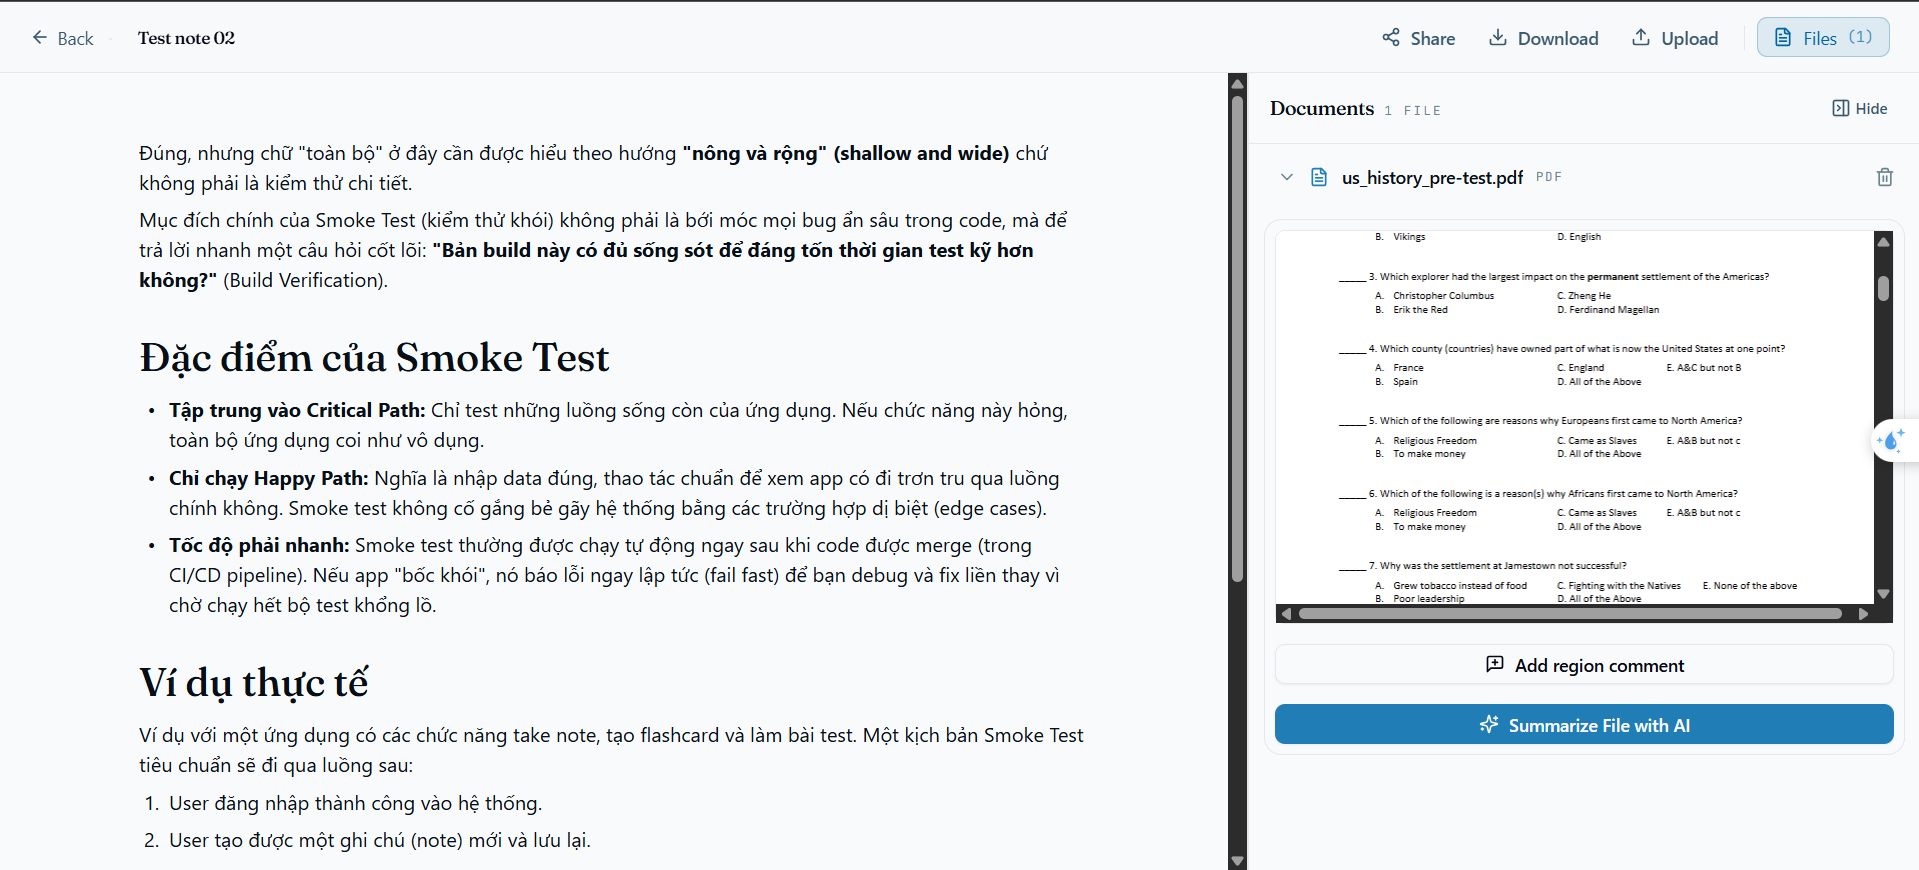
\includegraphics[width=\linewidth]{images/Feature/Web/Note_Web.png}
            \caption{Giao diện Web - Ghi chép kết hợp tài liệu}
        \end{minipage}\hfill
        \begin{minipage}{0.48\textwidth}
            \centering
            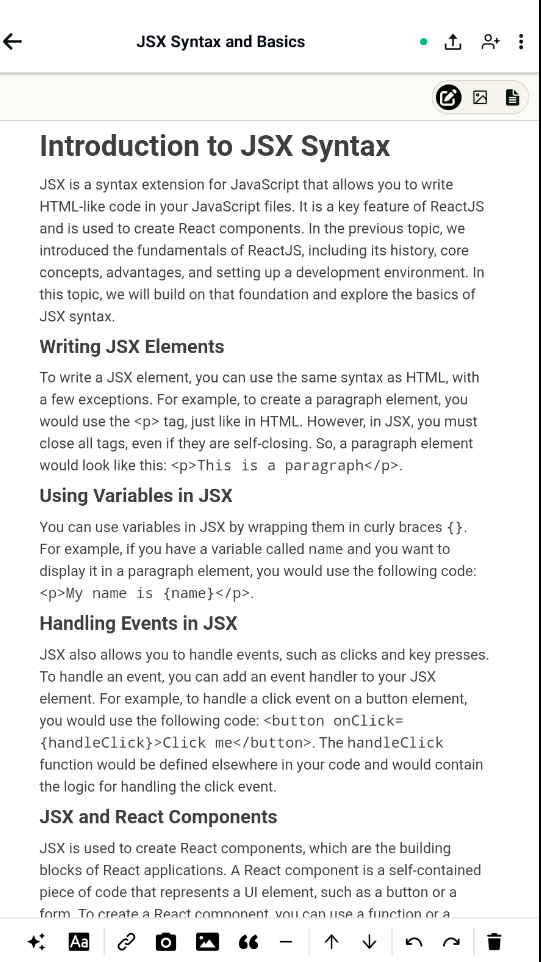
\includegraphics[width=\linewidth]{images/Feature/Mobile/Note_Mobile.png}
            \caption{Giao diện Mobile - Ghi chép kết hợp tài liệu}
        \end{minipage}
        \label{fig:note_taking}
    \end{figure}

    \item \textbf{Tạo Flashcard (Thủ công hoặc AI):} Người học có thể tạo thủ công hoặc tải học liệu có sẵn để AI tự động sinh ra Flashcard (thẻ ghi nhớ, game ghép thẻ. Đồng thời hệ thống cũng có chế độ nhắc nhở người dùng ôn luyện những card chưa vững kiến thức.
    
    \begin{figure}[H]
        \centering
        \begin{minipage}{0.48\textwidth}
            \centering
            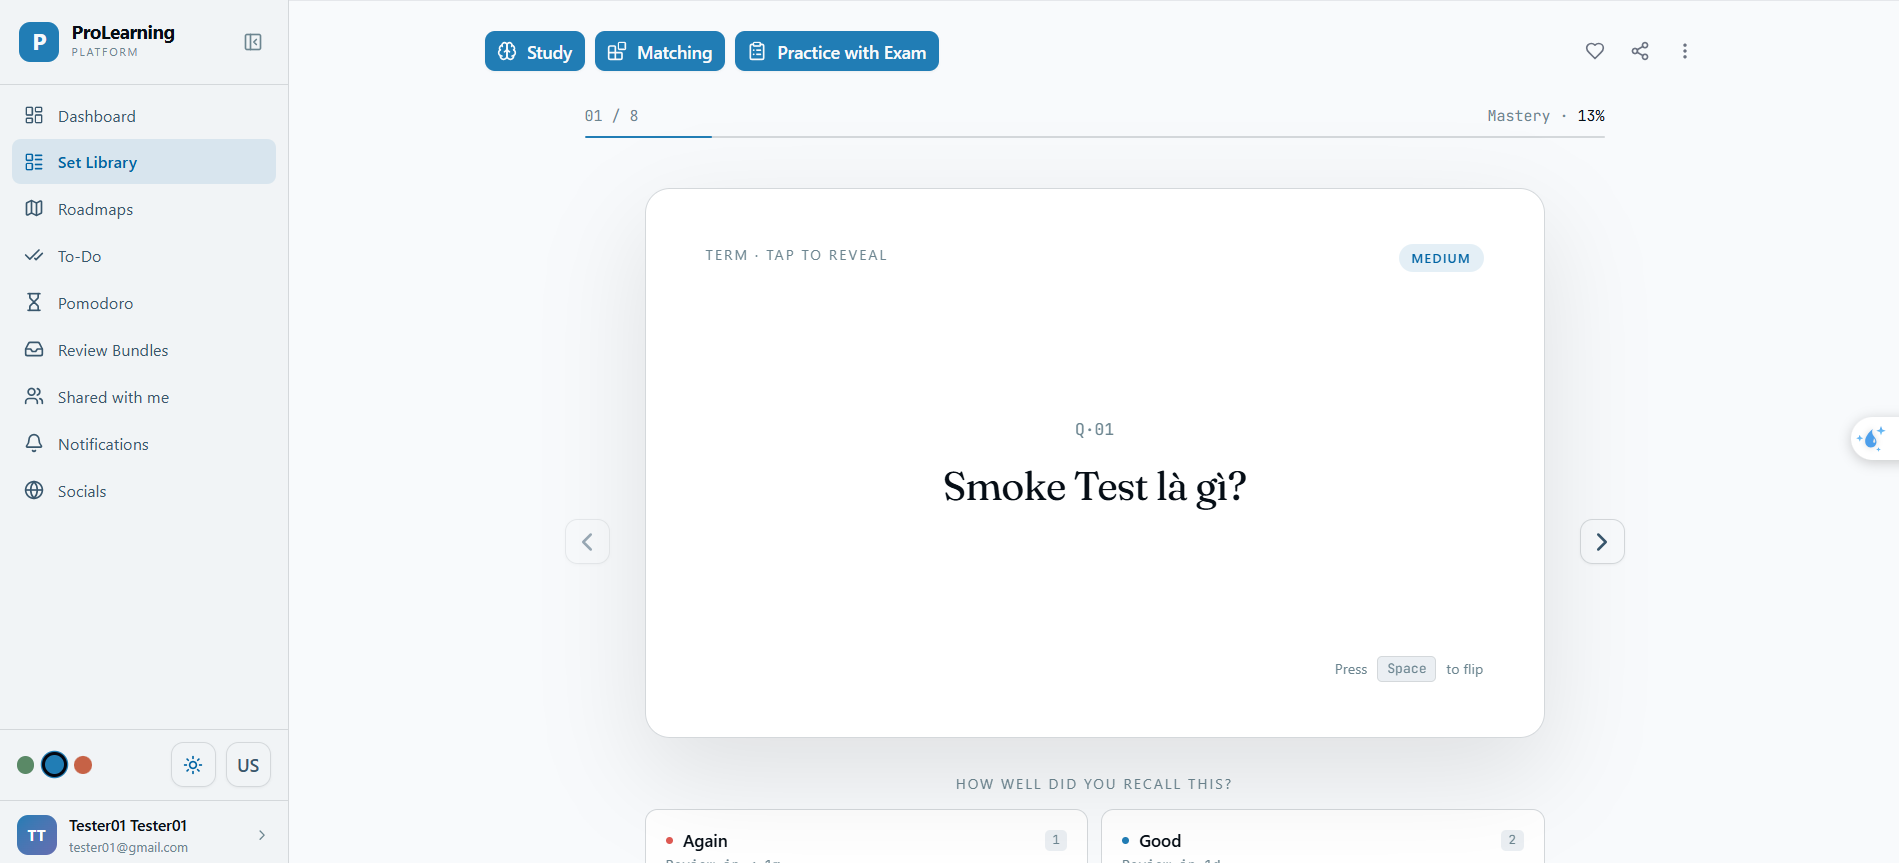
\includegraphics[width=\linewidth]{images/Feature/Web/Flashcard_Web.png}
            \caption{Giao diện Web - Flashcard}
        \end{minipage}\hfill
        \begin{minipage}{0.48\textwidth}
            \centering
            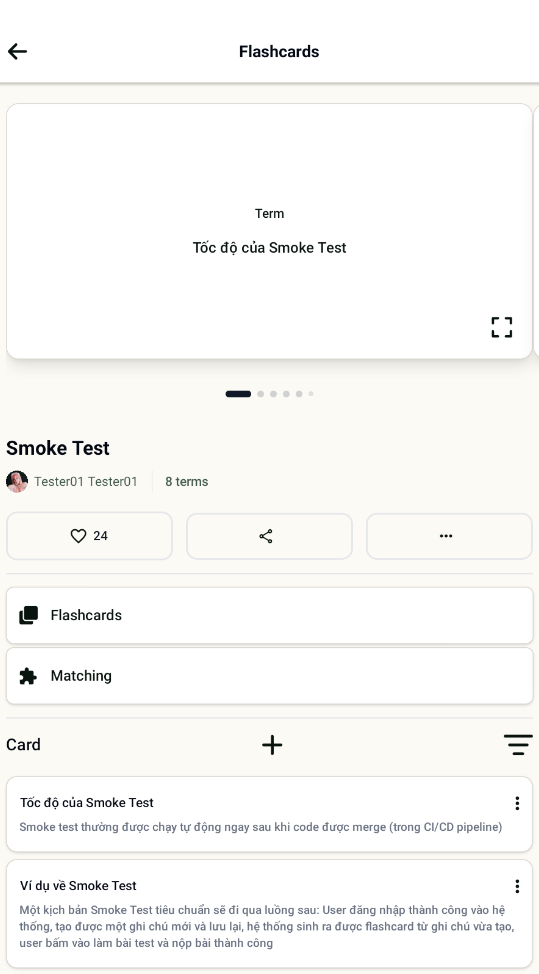
\includegraphics[width=\linewidth]{images/Feature/Mobile/Flashcard_Mobile.png}
            \caption{Giao diện Mobile - Flashcard}
        \end{minipage}
        \label{fig:quiz_flashcard}
    \end{figure}

    \item \textbf{Tạo bài kiểm tra (Thủ công hoặc AI):} Hệ thống cho phép AI tự động chuyển đổi tài liệu học tập thành các bài kiểm tra đa dạng (trắc nghiệm, đúng/sai, điền câu trả lời). Tính năng này giúp đánh giá nhanh mức độ hiểu bài và cung cấp giải thích chi tiết cho từng câu trả lời. Đồng thời cũng có chức năng sinh ra bài kiểm tra dựa trên format của bài kiểm tra có sẵn.
    
    \begin{figure}[H]
        \centering
        \begin{minipage}{0.48\textwidth}
            \centering
            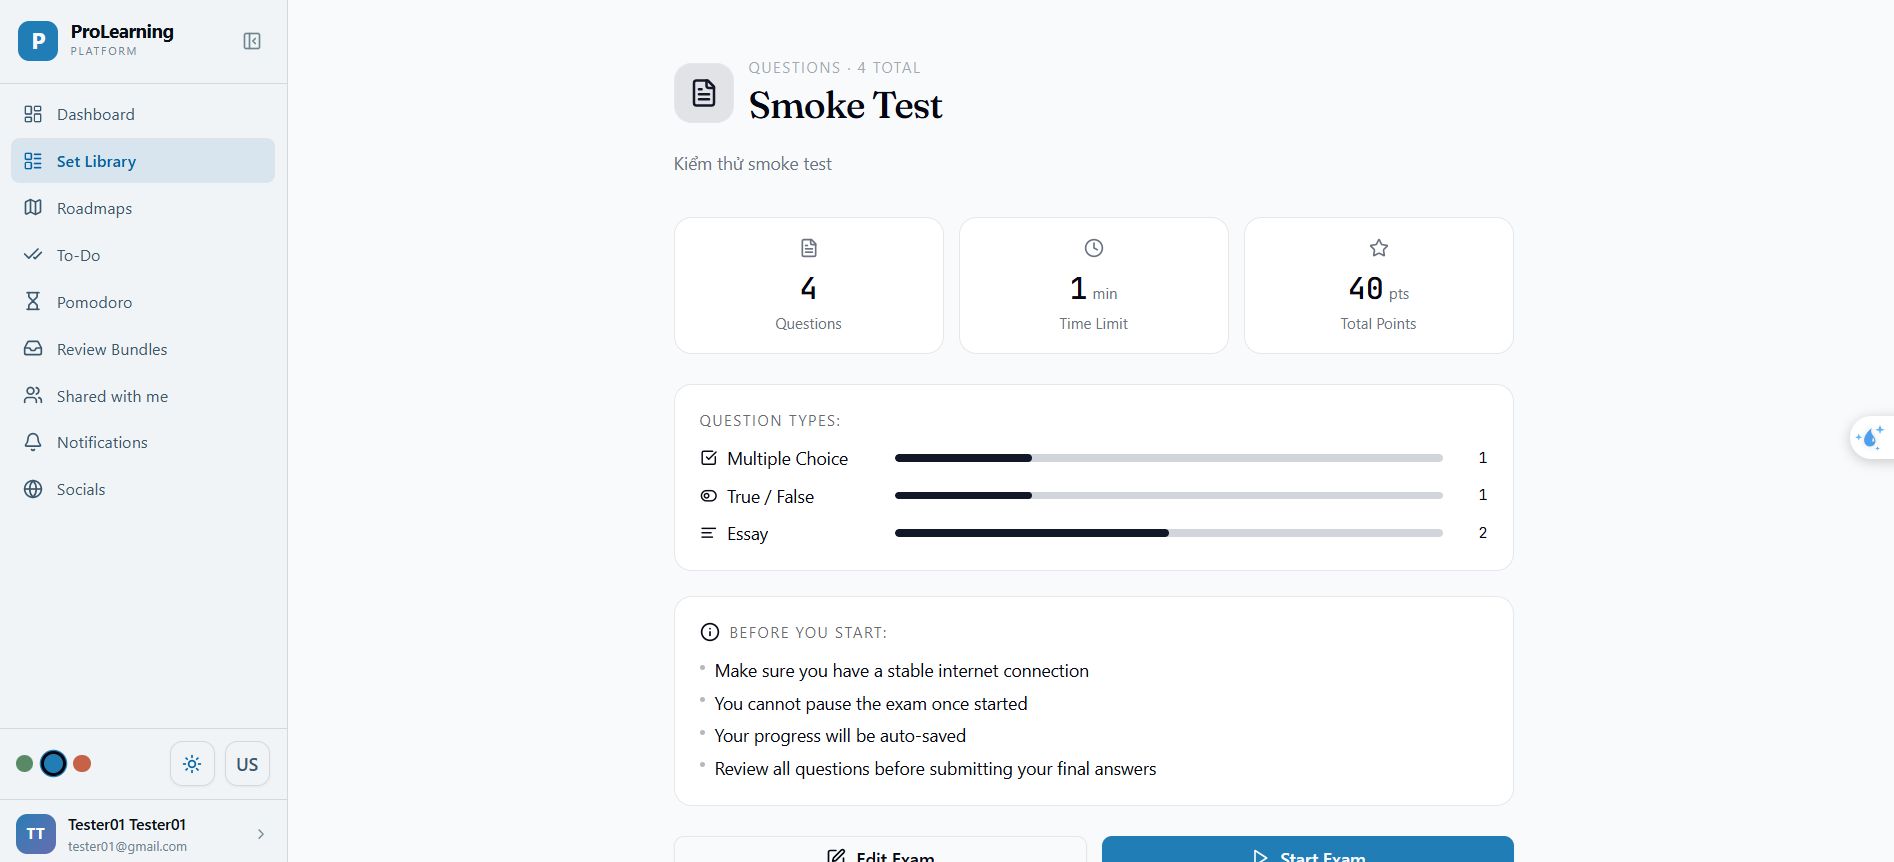
\includegraphics[width=\linewidth]{images/Feature/Web/Exam_Web.png}
            \caption{Giao diện Web - Bài kiểm tra}
        \end{minipage}\hfill
        \begin{minipage}{0.48\textwidth}
            \centering
            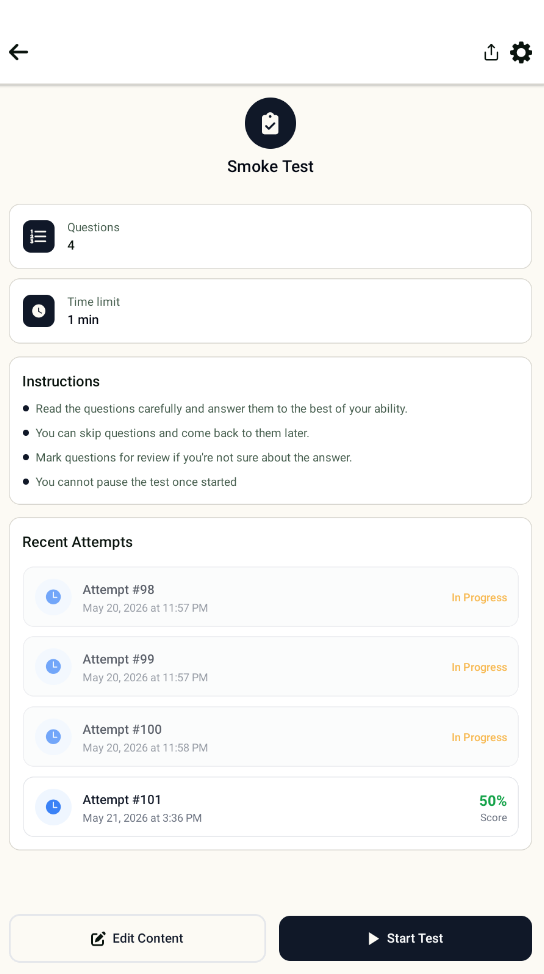
\includegraphics[width=\linewidth]{images/Feature/Mobile/Exam_Mobile.png}
            \caption{Giao diện Mobile - Bài kiểm tra}
        \end{minipage}
    \end{figure}

    \item \textbf{Xây dựng lộ trình học tập (Roadmap):} Dựa trên dữ liệu học tập và mục tiêu cá nhân, AI sẽ đề xuất một lộ trình học tập tối ưu. Roadmap giúp người dùng nắm bắt được các bước cần thực hiện để làm chủ kiến thức một cách khoa học.
    
    \begin{figure}[H]
        \centering
        \begin{minipage}{0.48\textwidth}
            \centering
            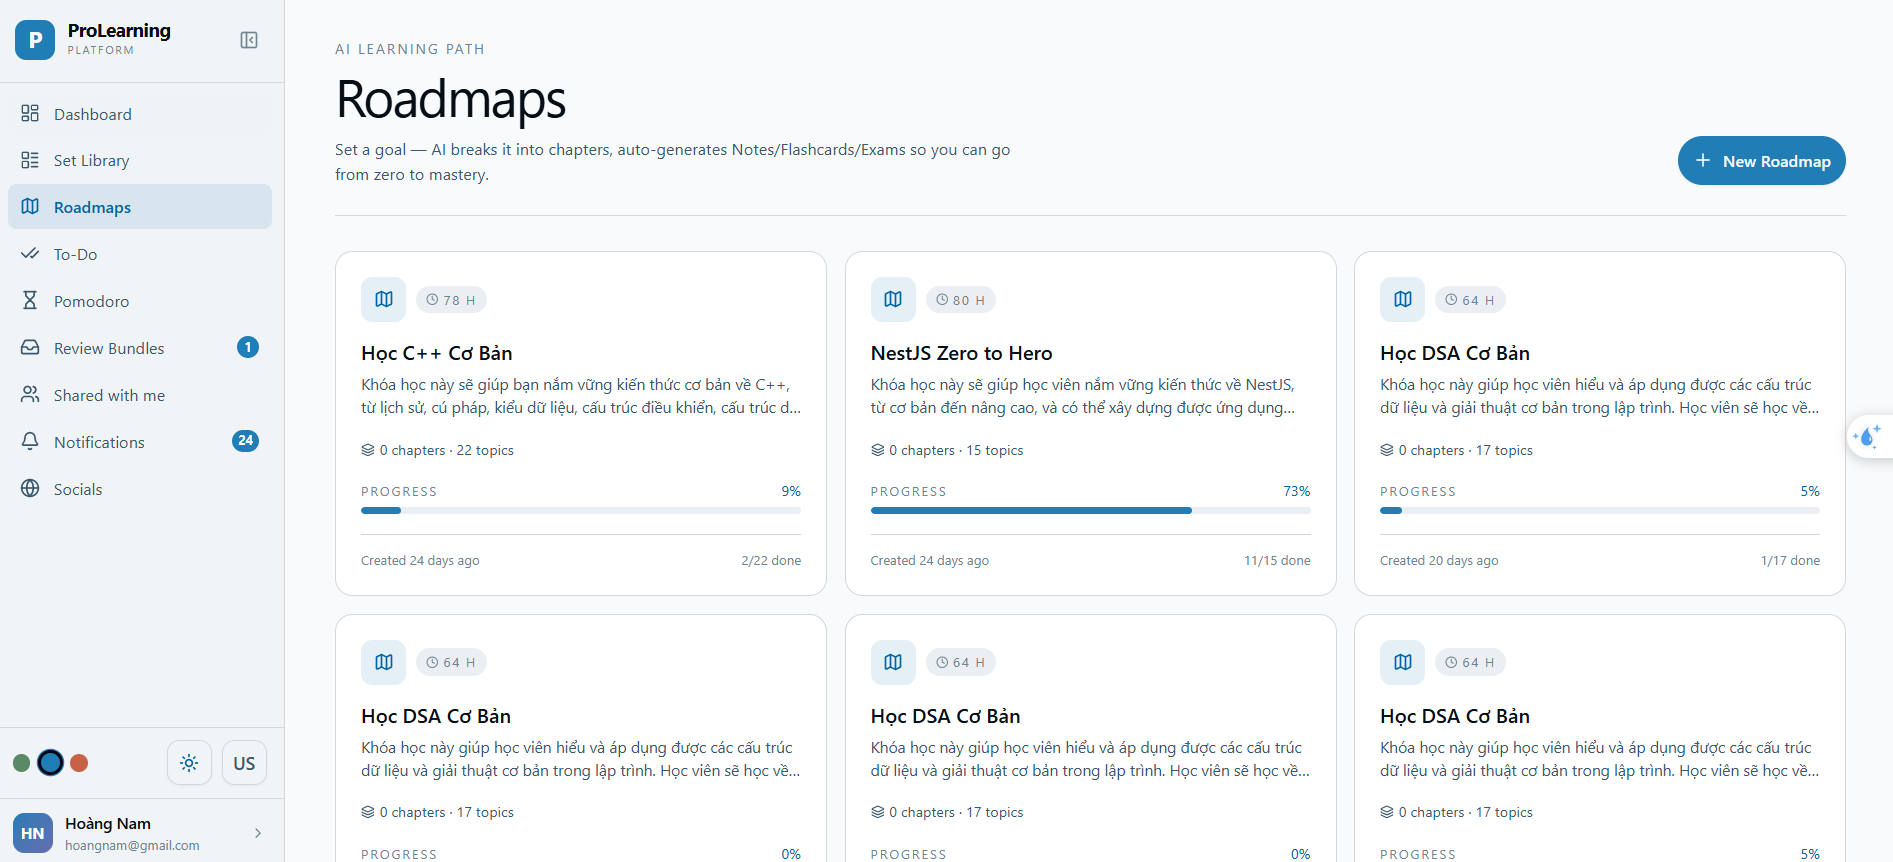
\includegraphics[width=\linewidth]{images/Feature/Web/Roadmap_Web.png}
            \caption{Giao diện Web - Lộ trình học tập}
        \end{minipage}\hfill
        \begin{minipage}{0.48\textwidth}
            \centering
            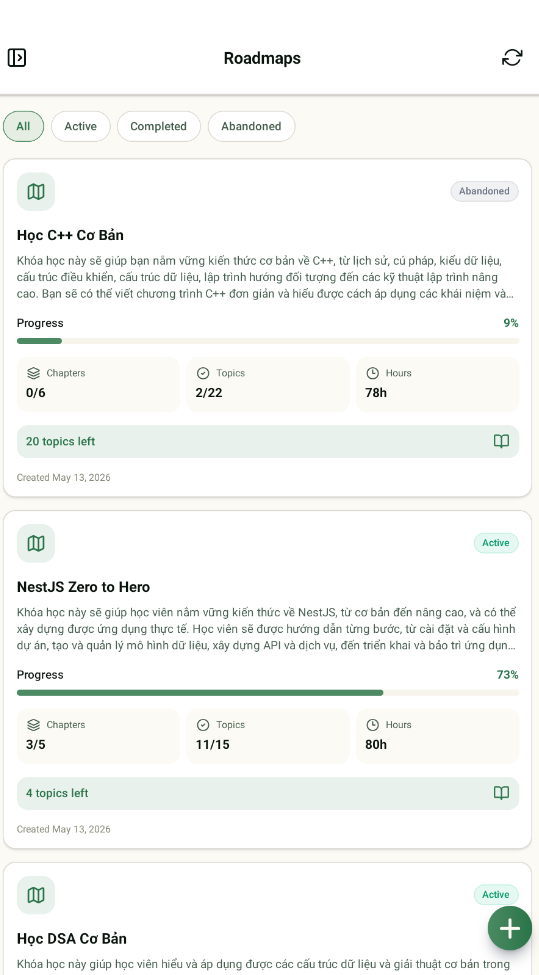
\includegraphics[width=\linewidth]{images/Feature/Mobile/Roadmap_Mobile.png}
            \caption{Giao diện Mobile - Lộ trình học tập}
        \end{minipage}
    \end{figure}

    \item \textbf{Phân tích năng lực người học:} Hệ thống có chức năng phân tích năng lực của người học ở mỗi Flashcard, Exam và toàn bộ Set đó. Đánh giá điểm mạnh, điểm yếu và đè xuất hướng cải thiện.
    
    \begin{figure}[H]
        \centering
        \begin{minipage}{0.48\textwidth}
            \centering
            % Thay đường dẫn ảnh thực tế của bạn
            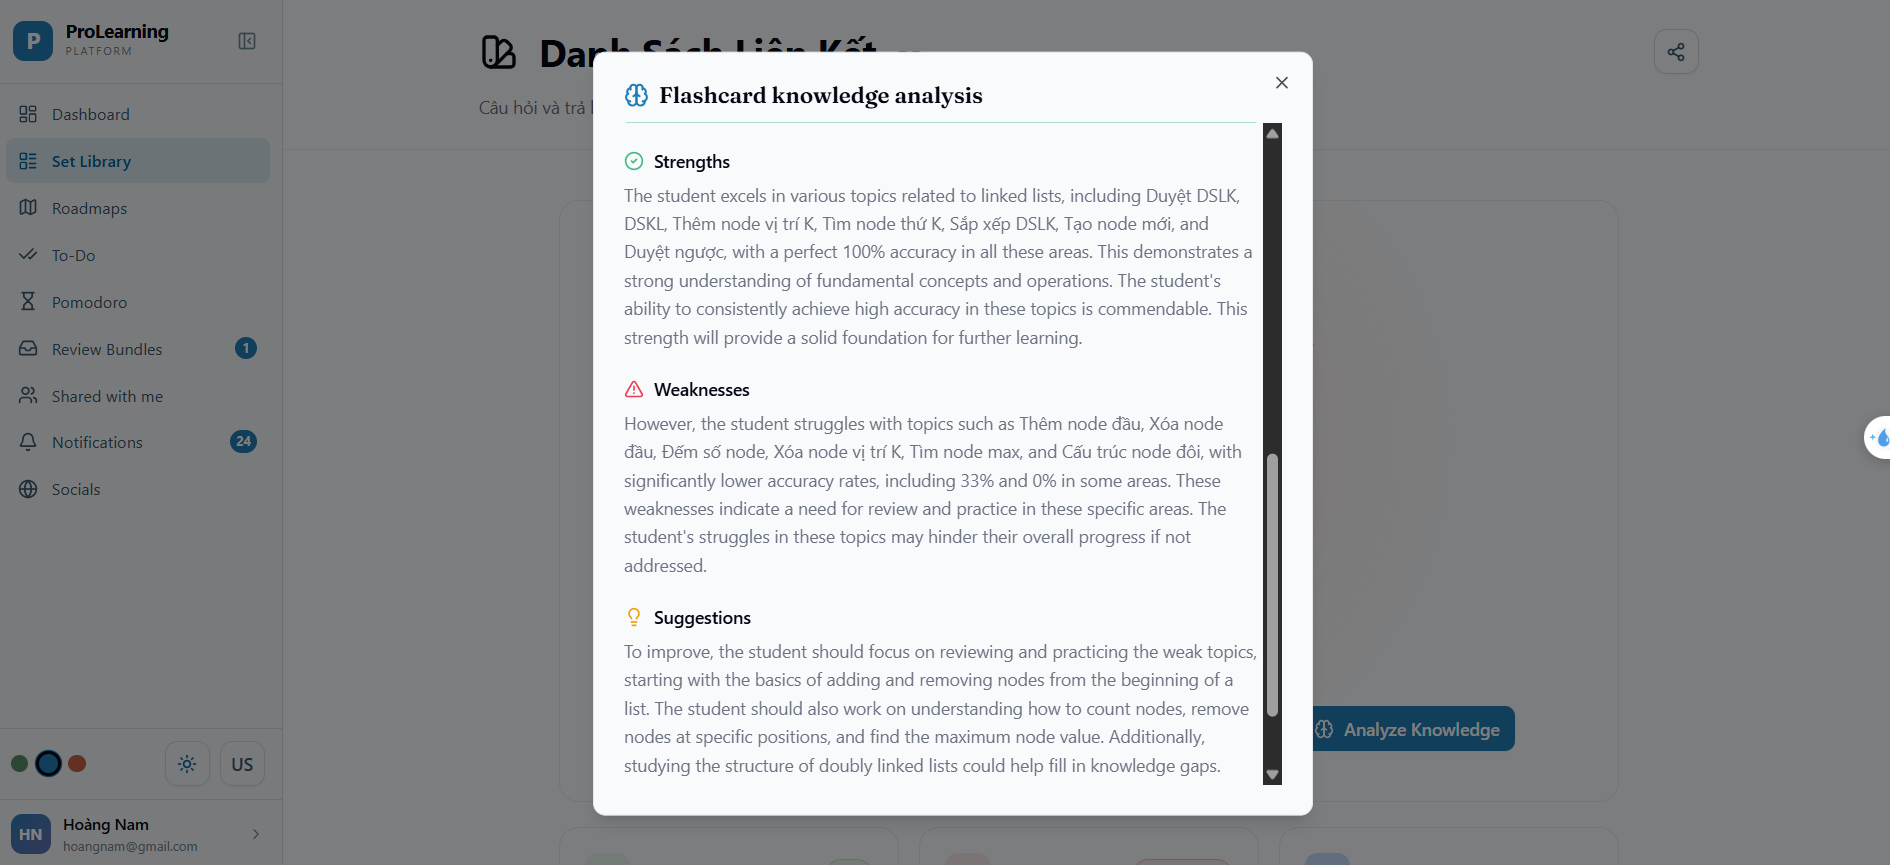
\includegraphics[width=\linewidth]{images/Feature/Web/Analysis_Web.png}
            \caption{Giao diện Web - Phân tích năng lực người học}
        \end{minipage}\hfill
        \begin{minipage}{0.48\textwidth}
            \centering
            % Thay đường dẫn ảnh thực tế của bạn
            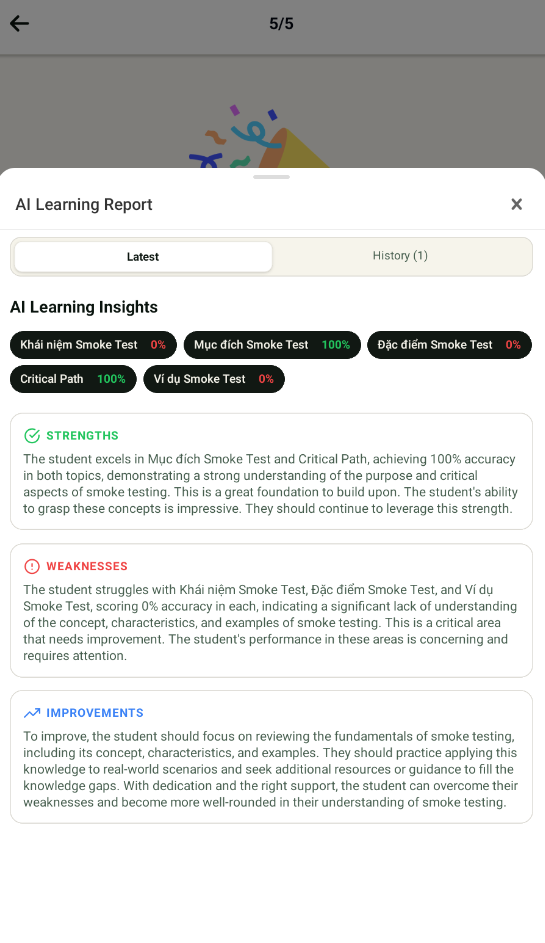
\includegraphics[width=\linewidth]{images/Feature/Mobile/Analysis_Mobile.png}
            \caption{Giao diện Mobile - Phân tích năng lực người học}
        \end{minipage}
    \end{figure}

    \item \textbf{Quản lý Task và Trải nghiệm học:} Tích hợp các công cụ quản lý thời gian như To-do list và bộ đếm Pomodoro. Tính năng này giúp người học duy trì sự tập trung, theo dõi tiến độ công việc và cá nhân hóa trải nghiệm học tập hàng ngày.
    
    \begin{figure}[H]
        \centering
        \begin{minipage}{0.48\textwidth}
            \centering
            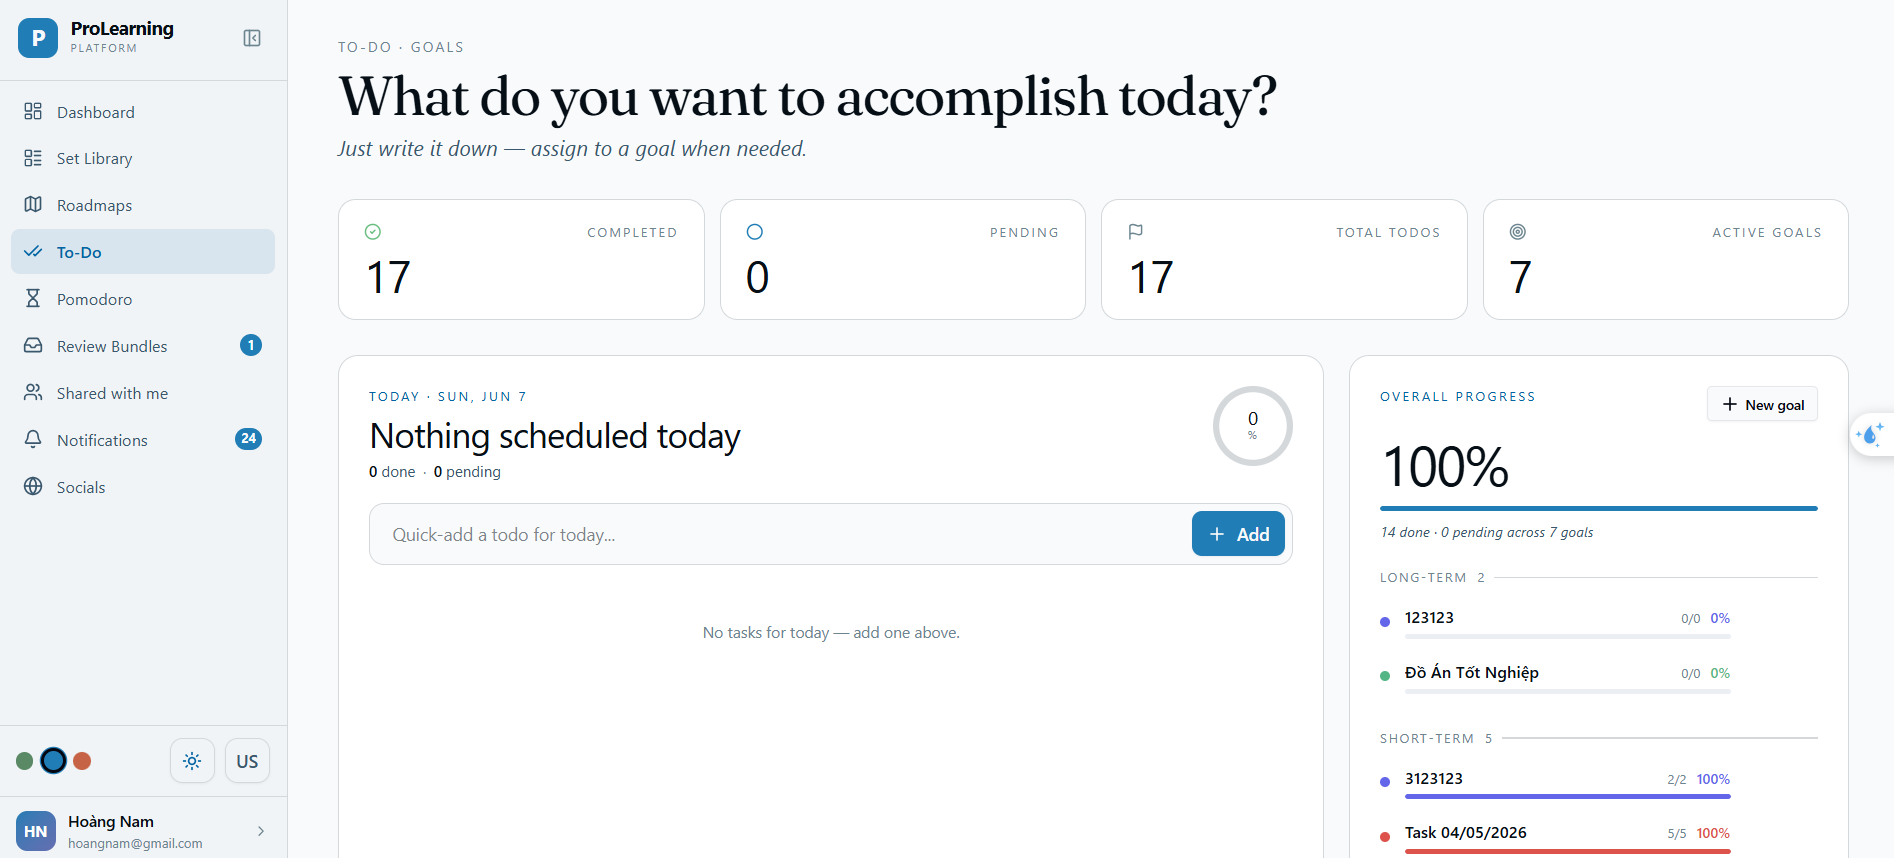
\includegraphics[width=\linewidth]{images/Feature/Web/ToDoList_Web.png}
            \caption{Giao diện Web - Quản lý Task}
        \end{minipage}\hfill
        \begin{minipage}{0.48\textwidth}
            \centering
            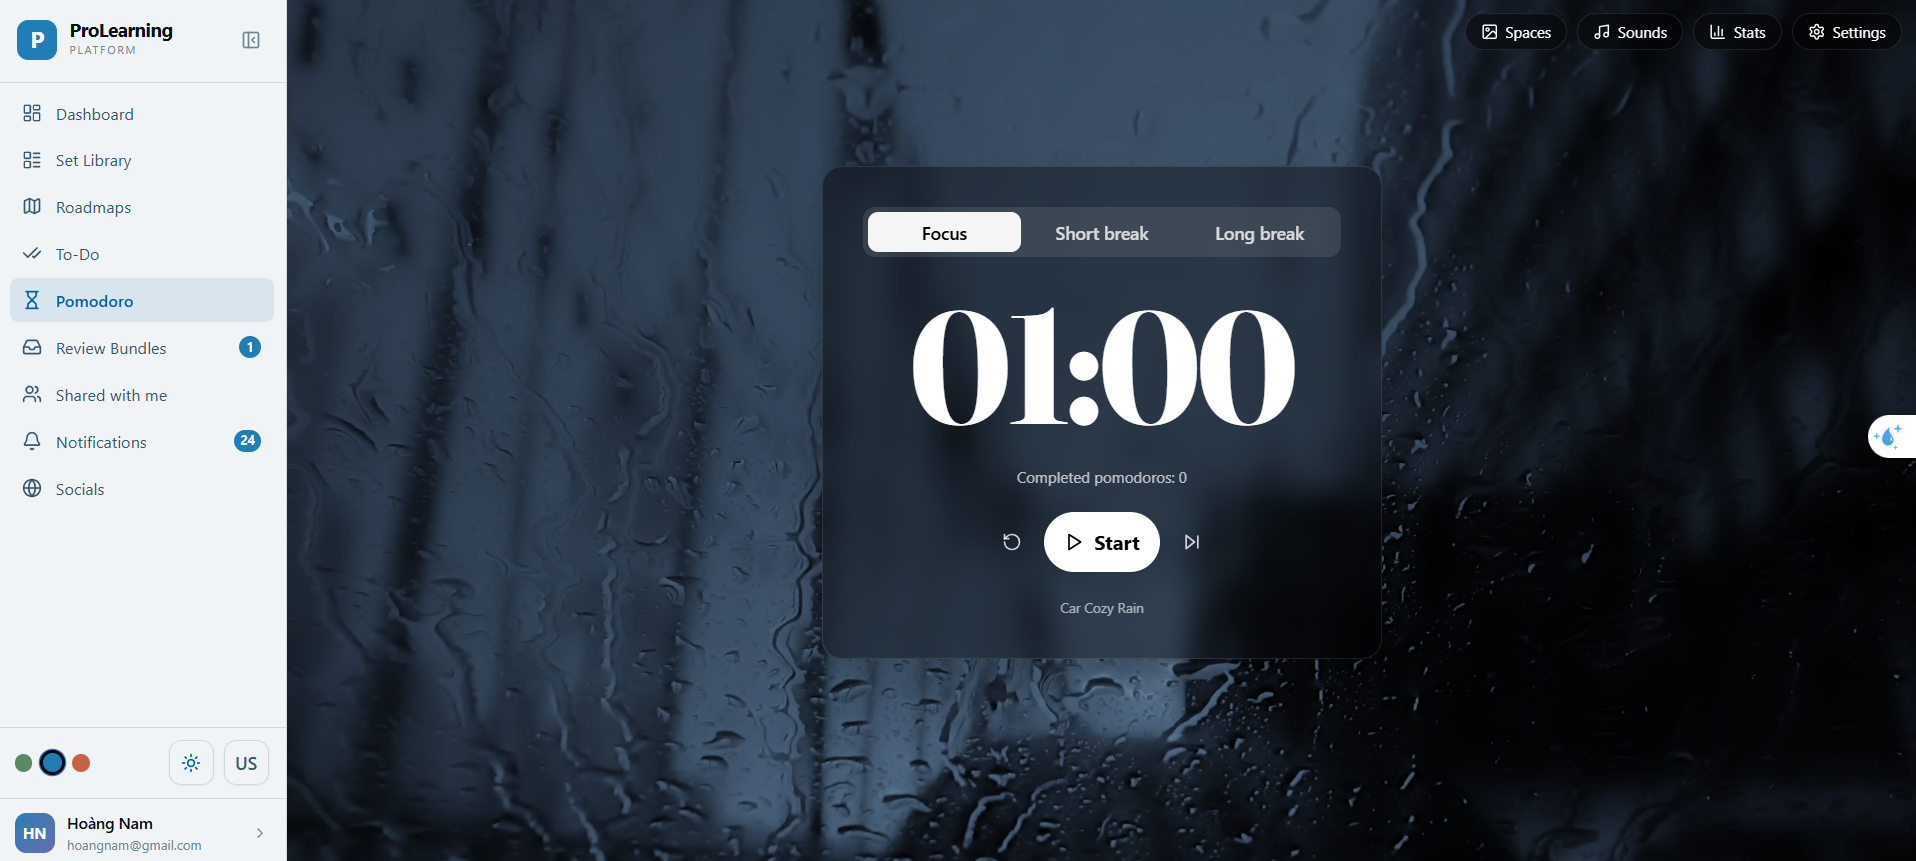
\includegraphics[width=\linewidth]{images/Feature/Web/Pomodoro_Web.png}
            \caption{Giao diện web - Pomodoro}
        \end{minipage}
    \end{figure}

    \begin{figure}[H]
        \centering
        \begin{minipage}{0.48\textwidth}
            \centering
            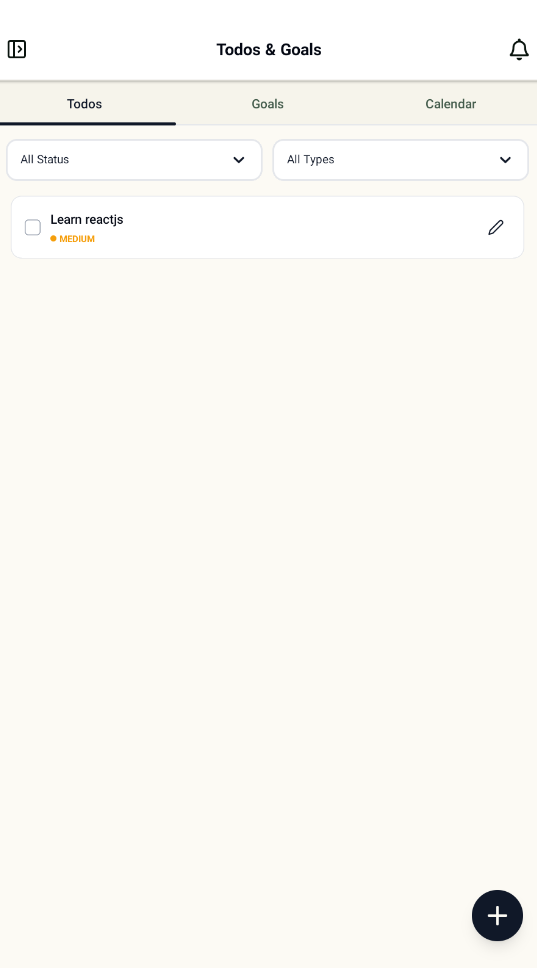
\includegraphics[width=\linewidth]{images/Feature/Mobile/ToDoList_Mobile.png}
            \caption{Giao diện Mobile - Quản lý Task}
        \end{minipage}\hfill
        \begin{minipage}{0.48\textwidth}
            \centering
            
\includegraphics[width=\linewidth]{images/Feature/Mobile/Pomodoro_Mobile.png}
            \caption{Giao diện Mobile - Pomodoro}
        \end{minipage}
    \end{figure}

\end{itemize}


\subsection{Đánh giá chức năng hệ thống}

Bên cạnh việc kiểm thử theo từng luồng chức năng trong quá trình phát triển, nhóm tổng hợp các chức năng chính của hệ thống để đánh giá mức độ hoàn thiện sau khi triển khai. Bảng~\ref{tab:function-evaluation-1} và Bảng~\ref{tab:function-evaluation-2} là mẫu đánh giá chức năng của hệ thống ProLearning Platform.

\begin{table}[H]
\centering
\caption{Bảng đánh giá chức năng hệ thống}
\label{tab:function-evaluation-1}
\small
\begin{tabular}{|L{0.20\textwidth}|L{0.62\textwidth}|C{0.11\textwidth}|}
\hline
\textbf{Tính năng} & \textbf{Mô tả} & \textbf{Mức đánh giá} \\
\hline
Xác thực người dùng & Hệ thống hỗ trợ đăng ký, đăng nhập, xác thực bằng JWT và duy trì phiên làm việc để người dùng truy cập các chức năng học tập cá nhân. & \textit{Tốt} \\
\hline
Kiểm soát truy cập và phân quyền & Hệ thống giới hạn quyền truy cập dữ liệu theo người dùng, vai trò và quyền sở hữu tài nguyên như note, flashcard set, todo hoặc subscription. & \textit{Tốt} \\
\hline
Quản lý học liệu và workspace & Người dùng có thể tổ chức học liệu theo không gian học tập, quản lý note, file, flashcard, exam và các tài nguyên liên quan. & \textit{Tốt} \\
\hline
Ghi chú thông minh kết hợp tài liệu & Hệ thống cho phép ghi chú kết hợp tài liệu, hỗ trợ tải file và sử dụng AI để giải thích, tóm tắt hoặc trích xuất nội dung học tập. & \textit{Tốt} \\
\hline
Cộng tác thời gian thực trên ghi chú & Nhiều người dùng có thể cùng chỉnh sửa ghi chú, đồng bộ nội dung, cursor và presence thông qua WebSocket/STOMP và Yjs. & \textit{Tốt} \\
\hline
Tạo flashcard thủ công hoặc bằng AI & Người dùng có thể tạo flashcard thủ công hoặc yêu cầu AI sinh flashcard từ tài liệu, note, URL hoặc nội dung học tập có sẵn. & \textit{Tốt} \\
\hline
Ôn tập flashcard theo lịch cá nhân & Hệ thống hỗ trợ chọn card đến hạn, cập nhật trạng thái ghi nhớ và lên lịch ôn tập tiếp theo dựa trên thuật toán spaced repetition. & \textit{Tốt} \\
\hline
Tạo bài kiểm tra thủ công hoặc bằng AI & Hệ thống cho phép tạo exam thủ công hoặc dùng AI để sinh câu hỏi trắc nghiệm, đúng/sai, điền đáp án và giải thích câu trả lời. & \textit{Tốt} \\
\hline
\end{tabular}
\end{table}

\begin{table}[H]
\centering
\caption{Bảng đánh giá chức năng hệ thống (tiếp)}
\label{tab:function-evaluation-2}
\small
\begin{tabular}{|L{0.20\textwidth}|L{0.62\textwidth}|C{0.11\textwidth}|}
\hline
\textbf{Tính năng} & \textbf{Mô tả} & \textbf{Mức đánh giá} \\
\hline
Phân tích năng lực người học & Hệ thống tổng hợp kết quả học flashcard và exam để phân tích điểm mạnh, điểm yếu, mức độ nắm kiến thức và đề xuất hướng cải thiện. & \textit{Tốt} \\
\hline
Xây dựng lộ trình học tập & Dựa trên mục tiêu và dữ liệu học tập của người dùng, hệ thống sử dụng AI để đề xuất roadmap học tập phù hợp. & \textit{Tốt} \\
\hline
Quản lý todo và đồng bộ lịch & Người dùng có thể tạo todo, gán deadline, đặt độ ưu tiên và đồng bộ công việc với Google Calendar khi đã kết nối tài khoản. & \textit{Tốt} \\
\hline
Pomodoro và quản lý thời gian học & Hệ thống cung cấp bộ đếm Pomodoro để hỗ trợ người dùng tập trung, theo dõi phiên học và hình thành thói quen học tập. & \textit{Tốt} \\
\hline
Thông báo và nhắc nhở học tập & Hệ thống gửi notification trong ứng dụng và push notification cho các sự kiện như card đến hạn, todo, goal hoặc tổng kết học tập. & \textit{Tốt} \\
\hline
Thanh toán và nâng cấp tài khoản PRO & Hệ thống hỗ trợ tạo link thanh toán PayOS, xác minh webhook và kích hoạt tài khoản PRO sau khi giao dịch thành công. & \textit{Tốt} \\
\hline
Quản trị và kiểm duyệt nội dung & Admin có thể theo dõi, xử lý báo cáo, kiểm duyệt nội dung hoặc thực hiện các tác vụ quản trị cần thiết để vận hành hệ thống. & \textit{Tốt} \\
\hline
Đồng bộ dữ liệu giữa web và mobile & Dữ liệu học tập, tài khoản, thông báo và tiến độ của người dùng được đồng bộ thông qua backend để đảm bảo trải nghiệm nhất quán trên web và mobile. & \textit{Tốt} \\
\hline
\end{tabular}
\end{table}
% ============================================================
\section{Kiểm thử}
% ============================================================

Phần này trình bày kế hoạch và kết quả kiểm thử của hệ thống ProLearning Platform.

\subsection{Mục tiêu kiểm thử}

Mục tiêu của quá trình kiểm thử là xác nhận hệ thống đáp ứng đúng các yêu cầu chức năng và phi chức năng đã đặt ra. Cụ thể, quá trình kiểm thử tập trung vào các mục tiêu sau:

\begin{itemize}
    \item Đảm bảo các chức năng chính hoạt động đúng theo đặc tả yêu cầu.
    \item Đảm bảo dữ liệu người dùng được lưu trữ và đồng bộ chính xác giữa backend, web và mobile.
    \item Kiểm tra các luồng tích hợp với dịch vụ ngoài như AI Service, Firebase Cloud Messaging, Google Calendar và PayOS.
    \item Phát hiện lỗi giao diện, lỗi xử lý nghiệp vụ, lỗi phân quyền và lỗi phát sinh khi thao tác ở các trường hợp biên.
    \item Đánh giá mức độ ổn định của hệ thống trước khi triển khai và bàn giao.
\end{itemize}

\subsection{Phạm vi kiểm thử}

Phạm vi kiểm thử bao gồm các nhóm chức năng chính của hệ thống. Bảng~\ref{tab:test-scope} trình bày các nhóm chức năng cần kiểm thử và nội dung kiểm thử tương ứng.

\begin{table}[H]
\centering
\caption{Phạm vi kiểm thử hệ thống}
\label{tab:test-scope}
\small
\begin{tabular}{|L{0.28\textwidth}|L{0.70\textwidth}|}
\hline
\textbf{Nhóm chức năng} & \textbf{Nội dung kiểm thử} \\
\hline
Xác thực và phân quyền & Đăng ký, đăng nhập, đăng xuất, refresh token, truy cập tài nguyên theo quyền sở hữu và vai trò. \\
\hline
Workspace học tập & Tạo, cập nhật, xóa và truy xuất note, file, flashcard set, exam và các dữ liệu học tập liên quan. \\
\hline
Ghi chú và cộng tác realtime & Chỉnh sửa note, đồng bộ nội dung, hiển thị cursor/presence, lưu và khôi phục snapshot. \\
\hline
AI learning & Sinh flashcard, sinh exam, phân tích kiến thức và tạo roadmap từ dữ liệu học tập. \\
\hline
Flashcard review & Lấy danh sách card đến hạn, cập nhật kết quả học, tính lịch ôn tiếp theo và trạng thái card. \\
\hline
Todo, Pomodoro và Calendar & Quản lý todo, Pomodoro session, đồng bộ Google Calendar và xử lý thay đổi trạng thái công việc. \\
\hline
Notification & Tạo thông báo, hiển thị inbox, đánh dấu đã đọc, gửi push notification và xử lý device token không hợp lệ. \\
\hline
Thanh toán và subscription & Tạo payment link, xác minh webhook PayOS, cập nhật giao dịch và kích hoạt tài khoản PRO. \\
\hline
\end{tabular}
\end{table}

\subsection{Chiến lược kiểm thử}

Nhóm áp dụng kết hợp nhiều hình thức kiểm thử nhằm bao phủ cả backend, web và mobile:

\begin{itemize}
    \item \textbf{Kiểm thử chức năng:} Kiểm tra từng chức năng theo các luồng sử dụng chính và các trường hợp biên.
    \item \textbf{Kiểm thử API:} Gọi trực tiếp các endpoint backend để kiểm tra request, response, mã lỗi và phân quyền.
    \item \textbf{Kiểm thử tích hợp:} Kiểm tra các flow có nhiều thành phần phối hợp như AI Service, WebSocket, Google Calendar, FCM và PayOS.
    \item \textbf{Kiểm thử giao diện:} Kiểm tra khả năng hiển thị, điều hướng, nhập liệu và phản hồi lỗi trên web/mobile.
    \item \textbf{Kiểm thử hồi quy:} Sau khi sửa lỗi hoặc thêm tính năng mới, kiểm tra lại các luồng chính để tránh phát sinh lỗi cũ.
\end{itemize}

\subsection{Kiểm thử tích hợp với dịch vụ ngoài}

Các chức năng phụ thuộc dịch vụ ngoài cần được kiểm thử riêng vì có thể phát sinh lỗi do timeout, sai cấu hình, token hết hạn hoặc dữ liệu trả về không hợp lệ. Các trường hợp kiểm thử chính như sau:

\begin{itemize}
    \item \textbf{AI Service:} Kiểm tra sinh flashcard, sinh exam, phân tích kiến thức và tạo roadmap với dữ liệu đầu vào hợp lệ/không hợp lệ.
    \item \textbf{Firebase Cloud Messaging:} Kiểm tra gửi push notification, cập nhật trạng thái gửi và xóa token không hợp lệ.
    \item \textbf{Google Calendar:} Kiểm tra OAuth callback, lưu credential, tạo/cập nhật/xóa event tương ứng với todo.
    \item \textbf{PayOS:} Kiểm tra tạo payment link, xác minh chữ ký webhook, xử lý webhook trùng lặp và kích hoạt PRO idempotent.
    \item \textbf{Cloudinary và dịch vụ lưu trữ file:} Kiểm tra upload, truy xuất và xóa file/tài nguyên liên quan nếu có.
\end{itemize}

\subsection{Kết quả kiểm thử}

Bảng~\ref{tab:test-result-summary} là tổng hợp kết quả kiểm thử theo từng nhóm chức năng chính của hệ thống.

\begin{table}[H]
\centering
\caption{Tổng hợp kết quả kiểm thử}
\label{tab:test-result-summary}
\small
\begin{tabular}{|L{0.22\textwidth}|C{0.10\textwidth}|C{0.10\textwidth}|C{0.10\textwidth}|L{0.34\textwidth}|}
\hline
\textbf{Nhóm chức năng} & \textbf{Số TC} & \textbf{Đạt} & \textbf{Không đạt} & \textbf{Ghi chú} \\
\hline
Xác thực và phân quyền & \textit{138} & \textit{138} & \textit{0} & \textit{Đăng nhập/đăng ký và phân quyền hệ thống về cơ bản hoạt động tốt} \\
\hline
Workspace học tập & \textit{180} & \textit{180} & \textit{0} & \textit{Workspace học tập với các set, flashcard, exam cũng như roadmap hoạt động tốt} \\
\hline
Các tool hỗ trợ học tập & \textit{90} & \textit{90} & \textit{0} & \textit{Các tool hỗ trợ học tập gồm Pomodoro, Todo \& Goal kết hợp Google Calendar hoạt động tốt} \\
\hline
AI learning & \textit{150} & \textit{150} & \textit{0} & \textit{Các chức năng AI hoạt động ổn định} \\
\hline
Realtime collaboration & \textit{30} & \textit{30} & \textit{0} & \textit{Tính năng cộng tác ghi chú và làm việc hoạt động bình thường} \\
\hline
Notification và scheduler & \textit{50} & \textit{50} & \textit{0} & \textit{Thông báo và nhắc nhở đầy đủ, không bị miss thông báo} \\
\hline
\end{tabular}
\end{table}

\subsection{Đánh giá sau kiểm thử}

Sau khi hoàn tất kiểm thử, nhóm tổng hợp các nhận xét chính về mức độ ổn định của hệ thống, các lỗi đã phát hiện và những hạn chế còn tồn tại. Kết quả đánh giá được trình bày trong Bảng~\ref{tab:post-test-evaluation}.

\begin{table}[H]
\centering
\caption{Đánh giá sau kiểm thử}
\label{tab:post-test-evaluation}
\small
\begin{tabular}{|L{0.16\textwidth}|L{0.40\textwidth}|L{0.32\textwidth}|}
\hline
\textbf{Nội dung đánh giá} & \textbf{Nhận xét} & \textbf{Hướng xử lý/cải thiện} \\
\hline
Các chức năng hoạt động ổn định & Các nhóm chức năng như xác thực và phân quyền người dùng, quản lý workspace, quản lý tài liệu học tập, Pomodoro, Roadmap và đồng bộ Google Calendar về cơ bản đáp ứng yêu cầu sử dụng. & Tiếp tục kiểm thử hồi quy khi bổ sung chức năng mới hoặc thay đổi API để đảm bảo các luồng chính không bị ảnh hưởng. \\
\hline
Các lỗi quan trọng đã phát hiện & Một số lỗi phát sinh ở các chức năng tích hợp với dịch vụ bên ngoài như Firebase Cloud Messaging, Google APIs hoặc các luồng phụ thuộc token/cấu hình môi trường. & Ghi nhận lỗi trên Trello, phân công thành viên phụ trách, kiểm tra lại cấu hình môi trường và bổ sung xử lý lỗi rõ ràng hơn ở backend/frontend. \\
\hline
Hạn chế còn tồn tại & Hệ thống còn phụ thuộc nhiều vào dịch vụ ngoài; bộ kiểm thử tự động chưa đầy đủ; chưa thực hiện sâu kiểm thử hiệu năng, kiểm thử tải và kiểm thử bảo mật. & Bổ sung automated test cho API và các luồng nghiệp vụ chính; xây dựng bộ regression test; lên kế hoạch kiểm thử performance/security trong các phiên bản tiếp theo. \\
\hline
\end{tabular}
\end{table}